\documentclass{article}[11pt]
\usepackage{xparse}
\usepackage{fancyhdr}
\usepackage{pgf,tikz}
\usepackage[utf8]{inputenc}
\usepackage[T1]{fontenc}
\usepackage{listings}
\usepackage{xcolor}
\usepackage{graphicx}
\usepackage{amsmath}
\usepackage[a4paper,left=2cm,right=2cm,top=2.5cm,bottom=2cm]{geometry}
\usepackage{amsmath}
\usepackage{amssymb}
\usepackage{array}
\usepackage{pifont}
\usepackage{makecell}
\usepackage{xcolor}
\usepackage[]{algorithm2e}

% NEW COMMANDS & DEFINE
\definecolor{pythonColor}{HTML}{B634F6}
\definecolor{codegreen}{rgb}{0,0.6,0}
\definecolor{codegray}{rgb}{0.5,0.5,0.5}
\definecolor{codered}{rgb}{1.0,0.2,0.2}
\definecolor{codeyellow}{rgb}{1.0,1.0,0.2}
\definecolor{codepurple}{rgb}{0.58,0,0.82}
\definecolor{backcolour}{rgb}{1.0,1.0,1.0}
\lstdefinestyle{mystyle}{
    backgroundcolor=\color{backcolour},
    commentstyle=\color{codepurple},
    keywordstyle=\color{magenta},
    numberstyle=\tiny\color{codegray},
    stringstyle=\color{codepurple},
    basicstyle=\ttfamily\footnotesize,
    breakatwhitespace=true,
    breaklines=true,
    % captionpos=b,
    keepspaces=true,
    numbers=left,
    numbersep=10pt,
    showspaces=false,
    showstringspaces=false,
    showtabs=false,
    tabsize=2,
    frame=false
}

\lstset{style=mystyle}
\newcommand{\python}[1]{\textcolor{pythonColor}{\textit{#1}}}
\renewcommand{\headrulewidth}{0.5pt}
\renewcommand{\footrulewidth}{0.5pt}
\newcommand{\showCode}[1]{\lstinputlisting[language=Python]{#1}}


% DOCUMENTS SETTINGS
\newcommand{\titre}{Factorisations matricielles}
\newcommand{\devoir}{Analyse Numérique : Devoir 2}
\newcommand{\auteur}{Romain Graux}
\newcommand{\noma}{28681700}
\newcommand{\mytitle}{
    \raggedbottom
    \lhead{\auteur}
    \rhead{Novembre 2019}
    \lfoot{28681700}
    \rfoot{\titre}
    \pagestyle{fancy}
    \begin{center}
        \huge{{\textbf{\devoir}}}

        \Huge{\textit{\textbf{\titre}}}
    \end{center}
    \vspace{0.7cm}
}

\graphicspath{./res/plots/}
\pagestyle{plain}

\begin{document}
\mytitle
\section{LU}

\subsection{Factorisation}
Cette décomposition a pour but de factoriser la matrice initiale \python{A} en une matrice \textit{triangulaire inférieure} \python{L} à diagonale unité et une matrice \textit{triangulaire supérieure} \python{U} ainsi, {A = LU}.
Cette factorisation cherche d'abord a faire un \textit{pivotage partiel}, ainsi les lignes sont échangées pour mettre les éléments maximums contenus sous la diagonale sur l'élément de la diagonale, de cette manière on évitera par la suite de diviser par zéro lorsque l'on divisera par le pivot. Ensuite, on applique les \textit{éliminiations de Gauss} de manière itérative sur chaque éléments de \python{L} et de \python{U}. Comme nous sommes en Python, j'ai cherché à vectoriser un maximum de boucles, ce qui nous donne l'algorithme de 3 lignes suivant une fois la matrice pivotée:
\lstinputlisting[language=Python, firstline=3, lastline=11]{res/py/LU.py}

\subsection{Résolution}
Nous appliquons d'abord la \textit{matrice de pivotage} (\python{P}) de chaque côté de l'équation $Ax=b$ ainsi, $PAx=Pb$.
Ensuite, ayant \python{LU} comme étant deux \textit{matrices triangulaires}, nous pouvons résoudre de la manière suivante en appliquant pour la résolution avec \python{L}, une substitution avant et avec \python{U}, une substitiution arrière, de la manière suivante:
\begin{align*}
     Ax&=b \\
    PAx& =Pb && \text{Multiplication par la matrice de permutation } P\\
    LUx& =Pb && \text{Factorisation } LU \text{ de la matrice } PA\\
    Ly& =Pb && \text{Résolution de } y \text{ par substitution avant}\\
    Ux&=y && \text{Résolution de } x \text{ par substitution arrière}
\end{align*}

\subsection{Propriétés}
\textbf{Déterminant}: Le déterminant d'un produit est le produit des déterminants, ainsi : $det(A)=det(PLU)=det(P)det(L)det(U)$ hors :
\begin{itemize}
    \item[--] le déterminant d'une \textit{matrice de permutation} vaut $-1^{p}$ avec p le nombre de permutations.
    \item[--] le déterminant d'une \textit{matrice triangulaire} est la multiplication des éléments de sa diagonale, de plus, $L$ a une diagonale unitaire, son déterminant vaut donc toujours $1$.
\end{itemize}
$\rightarrow$ Le déterminant de $A$ vaut donc simplement le produit des éléments diagonaux de $U$ multiplié par $-1$ si il y a un nombre impair de permuations ainsi : $det(A)=(-1)^{p}\prod_{i=1}^{m}U_{ii}$ \\
\noindent
\newline
\textbf{Inverse}:
Il y a deux techniques pour calculer l'inverse de \python{A}:
\begin{enumerate}
    \item L'inverse d'un produit est le produit des inverses en permutant le sens du produit, ainsi : $A^{-1}=(PLU)^{-1}=U^{-1}L^{-1}P^{-1}$ hors :
    \begin{itemize}
        \item[--] l'inverse d'une \textit{matrice de permutation} est sa \textit{transposée}.
        \item[--] l'inverse d'une \textit{matrice triangulaire supérieure} (resp. \textit{inférieure}) renvoie une \textit{matrice triangulaire supérieure} (resp. \textit{inférieure}), ainsi on peut se concentrer que sur une moitié de la matrice.
    \end{itemize}
    \item L'inverse de \python{A} peut être obtenue en resolvant le système $PLUA^{-1}=I_m$ hors :
        \begin{align*}
            PLUA^{-1}&=I_m \\
            LUA^{-1}&=P^T && \text{Comme sus-mentionné : }P^T=P^{-1}\\
            Ly&=P^T       && \text{Résolution par substitution avant}\\
            UA^{-1}&=y    && \text{Résolution par substitution arrière}\\
        \end{align*}
\end{enumerate}
\section{QR}
\subsection{Factorisation}
Cette factorisation a été réalisée autour d'une décomposition \textit{Gram–Schmidt modifié} car elle est plus stable que la classique dû aux erreurs d'arrondis.
Cette décomposition a pour but de factoriser la matrice initiale \python{A} en une matrice \python{Q} \textit{unitaire} et en une matrice \python{R} \textit{triangulaire supérieure} ainsi, {A = QR}.
\lstinputlisting[language=Python, firstline=3, lastline=13]{./res/py/QR.py}
\subsection{Résolution}
Ayant \python{Q} comme étant une matrice unitaire ($Q^{T}Q=I$), nous pouvons simplement obtenir la sous solution en multipliant par sa transposée. Ensuite \python{R} étant une matrice \textit{triangulaire supérieure}, nous pouvons obtenir la solution par \textit{substitution arrière}, de la manière suivante:
\begin{align*}
    Ax&=b \\
    QRx&=b && \text{Factorisation } QR \text{ de la matrice } A\\
    y&=Q^Tb && \text{Résolution de } y \text{ par multiplication de } Q^T\\
    Rx&=y && \text{Résolution de } x \text{ par substitution arrière}\\
\end{align*}
\section{Analyse}
\subsection{Complexité temporelle sur maillages différents}
\textbf{LU}: La complexité de \python{LUsolve} peut-être décomposée en deux parties:
\begin{itemize}
    \item[--] \python{LU}: Cette décomposition LU a une complexité temporelle de $\dfrac{2m^3}{3}$
    \item[--] \python{forward} \& \python{backward}: Les deux ont le même nombre d'opérations, prenons donc \python{forward}, elle va exécuter : $\sum_{i=1}^{m}\dfrac{b_i\sum_{j=1}^{i-1}A_{ij}x_{i}}{A_{ii}}$ ce qui est équivalent à une complexité pour les deux à la suite d'environ $2m^2$
    \item[] $\rightarrow$ Complexité totale $\sim \dfrac{2m^3}{3} + 2m^2 \sim \dfrac{2m^3}{3}$
\end{itemize}

\noindent
\textbf{QR}: La complexité de \python{QRsolve} peut également être décomposée en deux parties, la première est liée à la décomposition et vaut environ $\dfrac{4m^3}{3}$ et l'autre est liée à la résolution où la complexité est dominée par la substituion arrière elle même dominée par la décomposotion.
\begin{itemize}
    \item[] $\rightarrow$ Complexité totale $\sim \dfrac{4m^3}{3}$
\end{itemize}

\noindent\begin{minipage}{0.5\textwidth}
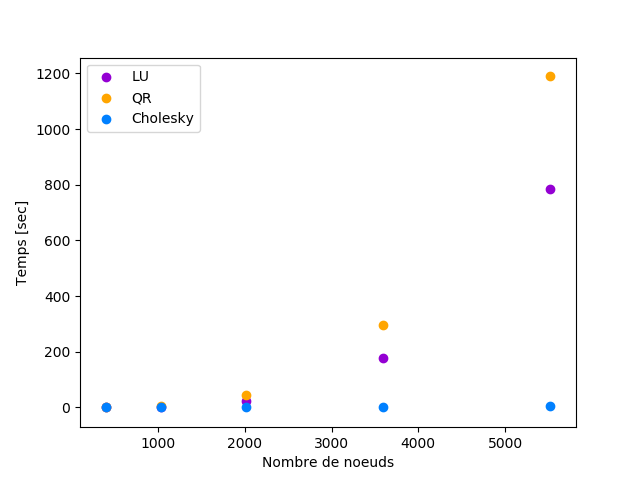
\includegraphics[width=\textwidth]{./res/plots/complexite.png}
\end{minipage}%
\begin{minipage}{0.5\textwidth}
Étant donné que la complexité de la \textit{factorisation LU} est de $\dfrac{2m^3}{3}$ et la complexité de la \textit{factorisation QR} est de $\dfrac{4m^3}{3}$ ($m$ étant la taille de la matrice A), il est normal d'observé que la résolution avec la \textit{factorisation LU} est plus rapide et les courbes suivent bien les complexités attendues.
\underline{Piste d'amélioration}: Étant donné que nous sommes en régime statique, la matrice \python{A} est symétrique et définie positive, il est possible d'utiliser une décomposition de \textit{Cholesky} qui a une complexitée deux fois moindre qu'une simple \textit{factorisation LU} puisqu'elle agit sur un triangle de la matrice symétrique. (Fonction \textit{Cholesky} de \textit{numpy})
\end{minipage}
\subsection{Complexité temporelle sur régimes différents}
\noindent\begin{minipage}{0.5\textwidth}
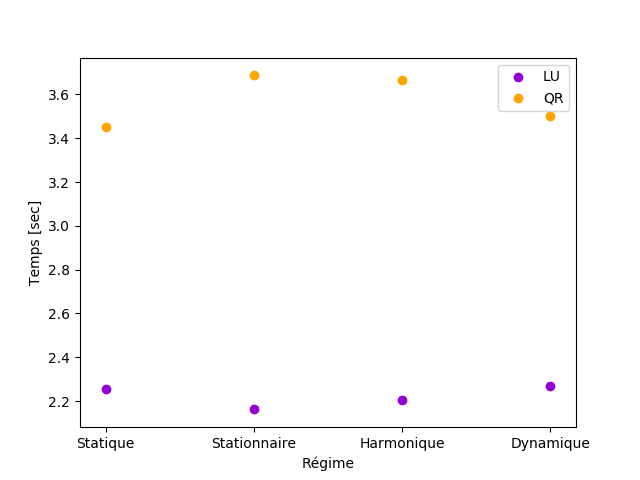
\includegraphics[width=\textwidth]{./res/plots/regimes.png}
\end{minipage}%
\begin{minipage}{0.5\textwidth}
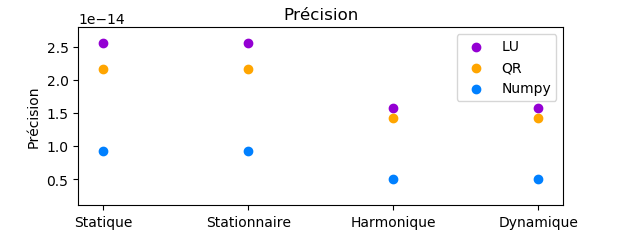
\includegraphics[width=\textwidth]{./res/plots/accuracyNumpy.png}
Comme expliqué au point [3.1], on peut observer que la complexité temporelle de \textit{QR} est environ deux fois supérieure à celle de \textit{LU}. Ensuite, ci-dessus nous pouvons observer que les deux décompositions ont une précision ($\dfrac{\norm{Ax-b}}{\norm{b}}$) proche de $10^{-14}$.
\end{minipage}

\subsection{Conditionnement ILU}
\noindent\begin{minipage}{0.5\textwidth}
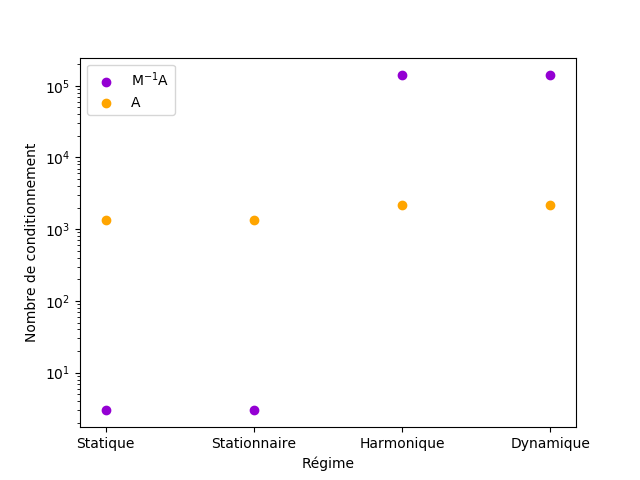
\includegraphics[width=\textwidth]{res/plots/conditionnementILU.png}
\end{minipage}%
\begin{minipage}{0.5\textwidth}
Comme nous pouvons l'observer, lorsque la \textit{vélocité} est égale de 0, la matrice $M^{-1}A$ est bien préconditionnée par rapport à la matrice initiale, cependant lorsque la \textit{vélocité} rentre en jeu, le conditionnement devient extrêmement plus grand dû aux termes dans A se rapprochant de 0 qui vont être divisé dans \textit{ILU}.
\end{minipage}


\end{document}
